%\section{Resummation of top quark mass-dependent logarithms at very high-energy via SCET}
\subsection{Resummation of top quark mass-dependent logarithms at high energy}
\label{sec:scet}

%\textit{Authors:} Sebastian Jaskiewicz, Stephen Jones, Robert Szafron, Yannick Ulrich (2501.00587)

\textbf{Sebastian Jaskiewicz, Stephen Jones, Robert Szafron, Yannick Ulrich~\cite{Jaskiewicz:2024xkd}.}


\noindent First steps in tackling the large top quark
mass scheme dependence that arises in this process,
as discussed at NLO in Section~\ref{sec:NLO-uncertainties}, were undertaken in~\cite{Jaskiewicz:2024xkd}. 
This study focused on investigating the 
high-energy behaviour of the $gg\to hh$ amplitude, namely the limit $s, |t|, |u| \gg m_t^2 \gg m_h^2$.
In this case, contributions due to the triangle
type diagrams in Fig.~\ref{fg:hhdia}
are power suppressed, and the dominant 
contribution arises from the box type diagrams.

The starting point of~\cite{Jaskiewicz:2024xkd} is
the observation that in the high-energy limit the
result for one- and two-loop box contributions in
the $\mathrm{OS}$ scheme has the structure
given in \eqref{eq:hhexp}.
Interestingly, the leading term proportional to the $C_F$ colour factor at two loops can be understood as originating from the mass renormalization counterterm. Indeed,
converting the top quark mass to the $\overline{{\rm{MS}}}$ scheme yields a logarithm of $\mu_t^2/s$~\cite{Baglio:2020ini},
as can explicitly be seen in~\eqref{eq:NLO-MSbar}.
Since the leading mass-dependent logarithm originates only from the mass renormalization counterterm, the leading behaviour of $F_\mathrm{box,i}^{(1)}$ in the small mass limit can be predicted solely from the leading order $F_\mathrm{box,i}^{(0)}$ result and the mass renormalization counterterm.
The immediate questions arising from this discussion
that were answered in~\cite{Jaskiewicz:2024xkd} are
\begin{enumerate}
    \item Why does the box amplitude have such a simple structure?
    \item Does this simple structure persist at higher orders, or can super-leading/power-enhanced terms enter in the integrals at higher loop orders to spoil this picture?
\end{enumerate}
The analysis carried out in~\cite{Jaskiewicz:2024xkd}
consists of two main parts.
First, a detailed fixed-order study is performed using
the Method of Regions (MoR) approach
\cite{Beneke:1997zp, Smirnov:1990rz, Smirnov:1994tg, Smirnov:2002pj}
investigating the modes and regions that contribute to the relevant
scalar integrals and to the amplitude. Second, an effective
field theory is constructed which formalizes the findings
from the MoR analysis to all orders in perturbation theory.
The relevant framework for the description of the
high-energy structure of the amplitude can be obtained using
Soft-Collinear Effective Field Theory (SCET) \cite{Bauer:2000yr, Bauer:2001yt,Bauer:2002nz, Beneke:2002ph, Beneke:2002ni},
which is suitable for processes with multiple collinear directions.
The upshot of this analysis is that it identifies, for $gg\to hh$ amplitudes at
high energies, the origin of the large logarithms
in $m_t^2/s$, which cause the discrepancy in the description of the
amplitude in the OS and $\overline{{\rm{MS}}}$ schemes.
Resummation of these large logarithms at leading-power
leading-logarithmic level is then shown to reduce
the mass scheme dependence of the amplitude at high energy.

The result of the investigations in Ref.~\cite{Jaskiewicz:2024xkd}
is that the all-order structure of the small top quark mass
power-expanded $y_t^2$ box contribution to the $gg \rightarrow hh$
amplitude can be written as follows in the $\overline{\mathrm{MS}}$ scheme
\begin{align}\label{eq:schem-lo}
& \mathrm{LO}: & &\alpha_s y_t^2 ( \textcolor{blue}{\boldsymbol{c_0}} + m_t \, n_0 ), & \\
& \mathrm{NLO}: & &\alpha_s^2 y_t^2  ( \textcolor{teal}{\boldsymbol{a_1 l_\mu}} + \textcolor{blue}{\boldsymbol{c_1}} + m_t \, n_1  ), & \\
& \mathrm{NNLO}: & &\alpha_s^3 y_t^2  ( \textcolor{teal}{\boldsymbol{a_2 l_\mu^2}} + \textcolor{orange}{\boldsymbol{b_2} \boldsymbol{l_m}} + \textcolor{blue}{\boldsymbol{c_2}} + m_t \, n_2 ), & \\
& \mathrm{N}^3\mathrm{LO}: & &\alpha_s^4 y_t^2 ( \textcolor{teal}{\boldsymbol{a_3 l_\mu^3}} + \textcolor{orange}{\boldsymbol{b_3} \boldsymbol{l_m^2}} + \textcolor{purple}{\boldsymbol{d_3 l_m}} + \textcolor{blue}{\boldsymbol{c_3}} + m_t \, n_3 ), & \\
%& & & \qquad \qquad \qquad \qquad \ldots & \nonumber \\
& \mathrm{N}^i\mathrm{LO}: &
&\alpha_s^{i-1} y_t^2 ( \textcolor{teal}{\boldsymbol{a_i l_\mu^i}} + \textcolor{orange}{\boldsymbol{b_i} \boldsymbol{l_m^{i-1}}}
+   \textcolor{purple}{\boldsymbol{
 d_i l_m^{i-2}}} + \ldots + \textcolor{blue}{\boldsymbol{c_i}} + m_t n_i ),&\label{eq:schem-nklo}
\end{align}
where $l_\mu = \ln(\mu_t^2/s)$ and $l_m$ contains both $\ln(\mu_t^2/s)$ and $\ln(m_t^2/s)$ logarithms. 
The $\textcolor{teal}{\boldsymbol{a_i l_\mu^i}}$ terms are the leading-power LLs, and they are known from the renormalization group running of the top quark mass.
The $\textcolor{orange}{\boldsymbol{b_i} \boldsymbol{l_m^{i-1}}}$ terms are the leading-power NLLs. These terms receive a contribution from the running of the top quark mass and from IR matching (massification)~\cite{Penin:2005eh, Mitov:2006xs, Becher:2007cu, Liu:2017axv, Engel:2018fsb, Wang:2023qbf, Wang:2024pmv}. The leading-power LLs depend on $\mu_t$, which can be set to the order of $\sqrt{s}$. This renders the explicit logarithms $l_\mu$ small. The dependence on the
large ratio of scales, $m_t^2/s$, is taken care of to all orders in the perturbative expansion implicitly through the running of the top quark mass. What drives the discrepancy discussed at NLO in Section~\ref{sec:NLO-uncertainties} is the fact that the conversion between the two schemes is truncated at NLO, so only the first logarithm in $m_t^2/s$ is captured in the OS scheme. In the study of Ref.~\cite{Jaskiewicz:2024xkd}, it was demonstrated that the origin of this
tower of logarithms is in fact known, and can be reinstated in the OS result
through
\begin{align}
A^{(j,\,{\text{LL}})}_{i,y_t^2}(m_t^\mathrm{OS}) = \left(\frac{m^{\text{LL}}(\mu_t)}{m_t^\mathrm{OS}} \right)^2 A^{(j)}_{i,y_t^2}(m_t^\mathrm{OS}), \label{eq:a_ll}
\end{align}
where
\begin{align}\label{eq:schmeme-conv-all-order}
    &m^{\text{LL}}(\mu) = M \exp \left[ a_{\gamma_m}^{\text{LL}}(\mu)\right]\, z_m(M),&
    &a_{\gamma_m}^{\text{LL}}(\mu) = \frac{3 C_F}{2 \beta_0} \ln \left(1 - \frac{\alpha_s(\mu)}{2 \pi} \beta_0 \ln \left(\frac{\mu^2}{M^2} \right) \right).&
\end{align}
The effect of including this tower of leading-power leading logarithms in the OS
result is demonstrated in Fig.~\ref{fig:all_sq_msbar_vs_osll}. As discussed above,
this study provides the first step in taming the top quark mass scheme uncertainty.
Thus far, the improvement can be seen at the level of the $gg\to hh$ amplitude in the
high-energy limit. Future studies are needed to tackle this sizeable uncertainty
in different regions of phase space and at the cross section level.



In future studies, it will be important to extend this analysis
from the amplitude level to physical observables, such as a
cross section, and beyond the high-energy limit. In order to
address the top quark mass scheme uncertainties at the total
cross section level, it is important to develop an understanding
of the uncertainty near the peak of the invariant mass distribution,
i.e.\ the region $300 \mathrm{GeV} < \sqrt{s} < 800 \mathrm{GeV}$,
which is a region that is not covered by the analysis carried out in
\cite{Jaskiewicz:2024xkd}.
One way of tackling this issue is to work out fully the subleading power
contributions, extending the region of validity of the high-energy framework.
For this, the basis has been developed in~\cite{Jaskiewicz:2024xkd}; however,
the factorization structure at subleading powers is much richer than the leading-power
counterpart, requiring, for example, the treatment of endpoint
divergences~\cite{Beneke:2020ibj,Beneke:2022obx,Liu:2019oav,Bell:2022ott}. Hence, it will be
interesting from both a theoretical and phenomenological point of view
to work on extending the framework of~\cite{Jaskiewicz:2024xkd} to next-to-leading power.
Alternatively, it can also be useful, if not necessary, to work on developing the all-order understanding of the structure of top quark mass corrections in a different expansion variable. For instance, it would be interesting to consider the HTL, the threshold expansion at $s \sim 4 m_t^2$, or the small-$p_T$ expansion.


\begin{figure}%[htbp]
     \centering
     \begin{subfigure}[b]{0.48\textwidth}
         \centering
         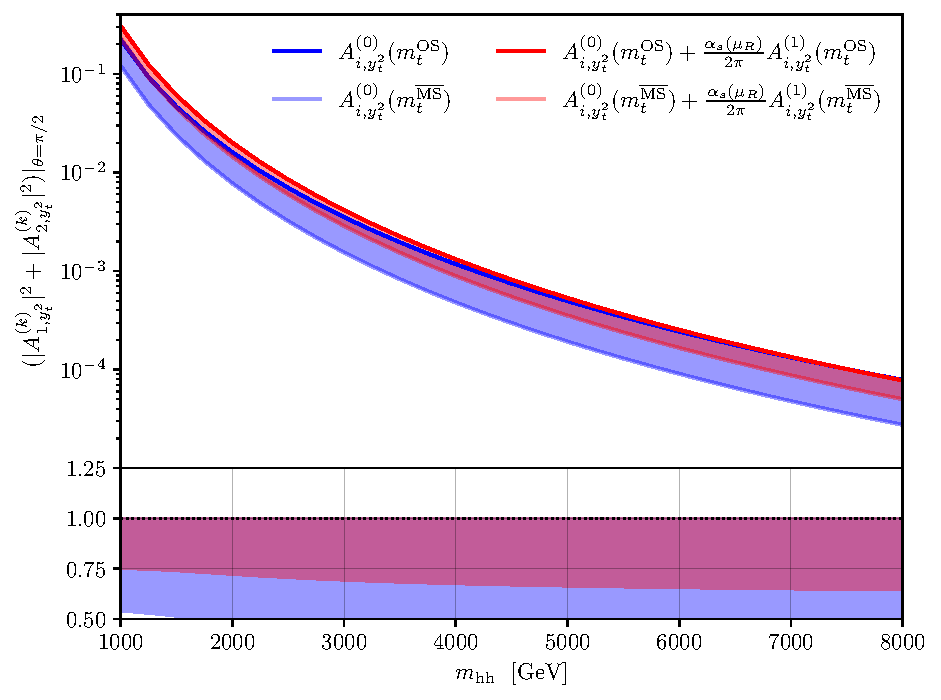
\includegraphics[width=\textwidth]{mt_UN/mt_LP_LL/Images/all_sq_amplitude_os_uncert-v1loop_mhh.pdf}
         \caption{ }
         \label{sfig:all_sq_msbar_vs_os}
     \end{subfigure}
     \hfill
     \begin{subfigure}[b]{0.48\textwidth}
         \centering
         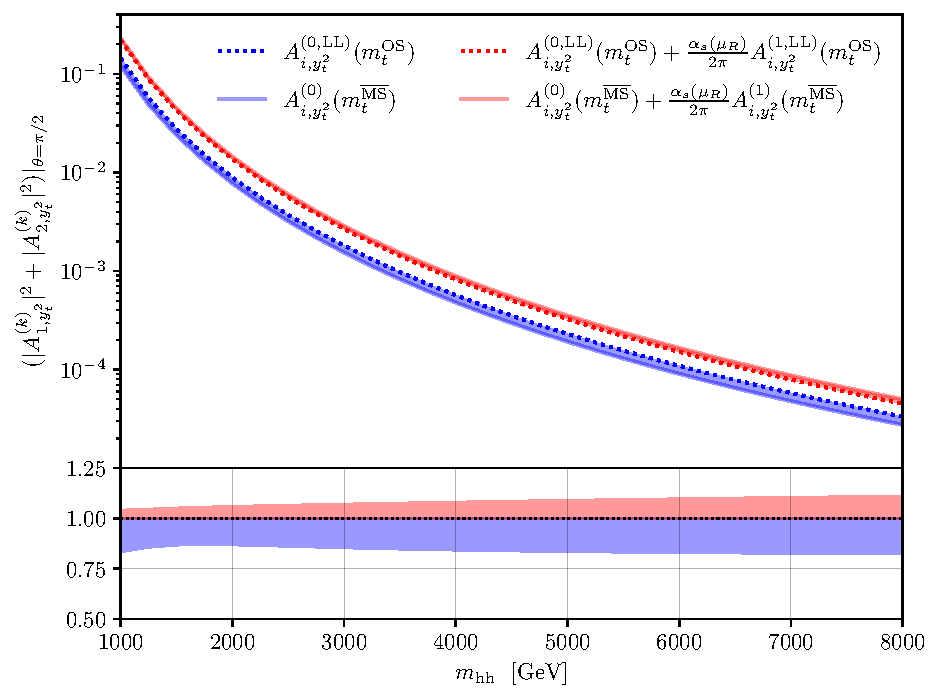
\includegraphics[width=\textwidth]{mt_UN/mt_LP_LL/Images/all_sq_amplitude_osll_uncert-v1loop_mhh.pdf}
         \caption{}
         \label{sfig:all_sq_msbar_vs_osll}
     \end{subfigure}
        \caption{Comparison of results for the sum of the squared form factors at one- and
        two-loop order, where the top quark mass is renormalized in the $\overline{\mathrm{MS}}$
        and ${\mathrm{OS}}$ (see panel (a)), and the same quantities with the ${\mathrm{OS}}$
        result supplemented by the resummed tower of leading-power leading logarithms
        (see panel (b)). 
        A significant reduction in the size of the uncertainty due to the choice of the
        top quark mass renormalization scheme is observed. Results shown are from Ref.~\cite{Jaskiewicz:2024xkd}.}
        \label{fig:all_sq_msbar_vs_osll}
\end{figure}
